% !TeX program = pdfLaTeX
\documentclass[12pt]{article}
\usepackage{amsmath}
\usepackage{amsthm}
\usepackage{graphicx,psfrag,epsf}
\usepackage{enumerate}
\usepackage{natbib}
\usepackage{booktabs}
\usepackage{longtable}
\usepackage{array}
\usepackage{multirow}
\usepackage[table]{xcolor}
\usepackage{wrapfig}
\usepackage{float}
\usepackage{colortbl}
\usepackage{hyperref}
\usepackage{pdflscape}
\usepackage{tabu}
\usepackage{threeparttable}

\usepackage{url} % not crucial - just used below for the URL

%\pdfminorversion=4
% NOTE: To produce blinded version, replace "0" with "1" below.
\newcommand{\blind}{0}

% DON'T change margins - should be 1 inch all around.
\addtolength{\oddsidemargin}{-.5in}%
\addtolength{\evensidemargin}{-.5in}%
\addtolength{\textwidth}{1in}%
\addtolength{\textheight}{1.3in}%
\addtolength{\topmargin}{-.8in}%

\newenvironment{definition}[1]% environment name 
{% begin code 
  \par\vspace{.75\baselineskip}\noindent 
  \textbf{Definition (#1)}\begin{itshape}% 
  \par\vspace{.5\baselineskip}\noindent\ignorespaces 
}% 
{% end code 
  \end{itshape}\ignorespacesafterend 
}

\providecommand{\tightlist}{%
  \setlength{\itemsep}{0pt}\setlength{\parskip}{0pt}}

\begin{document}

\def\spacingset#1{\renewcommand{\baselinestretch}%
{#1}\small\normalsize} \spacingset{1}


%%%%%%%%%%%%%%%%%%%%%%%%%%%%%%%%%%%%%%%%%%%%%%%%%%%%%%%%%%%%%%%%%%%%%%%%%%%%%%

\if0\blind
{
  \title{\bf Adaption of the Chumbley Score to matching of bullet striation marks}

  \author{
        Ganesh Krishnan \thanks{The authors gratefully acknowledge \ldots{}} \\
    Department of Statistics, Iowa State University\\
     and \\     Heike Hofmann \\
    Department of Statistics and csafe, Iowa State University\\
      }
  \maketitle
} \fi

\if1\blind
{
  \bigskip
  \bigskip
  \bigskip
  \begin{center}
    {\LARGE\bf Adaption of the Chumbley Score to matching of bullet striation marks}
  \end{center}
  \medskip
} \fi

\bigskip
\begin{abstract}

\end{abstract}

\noindent%
{\it Keywords:} 3 to 6 keywords, that do not appear in the title
\vfill

\newpage
\spacingset{1.45} % DON'T change the spacing!

\newcommand{\hh}[1]{{\textcolor{orange}{#1}}}
\newcommand{\gk}[1]{{\textcolor{green}{#1}}}
\newcommand{\cited}[1]{{\textcolor{red}{#1}}}

\tableofcontents

\section{Introduction and Background}\label{introduction-and-background}

\subsection{Problem statement and
motivation}\label{problem-statement-and-motivation}

\hh{'considered to be unique' by AFTE - that is right, but we should not use this argument, and I don't think we have to. It's better to focus on the problem at hand: striation marks are used to determine same source for bullets. XXX we could include some figures here XXX Current standards ask for a visual inspection of the marks under a comparison microscope by a firearms examiner. One of the problems raised by the NAS report in 2009 is the subjectivity involved in this comparison and the need for determining error rates \citep{NAS:2009}. There are different approaches used to achieve more objectivity and assess error rates. XXX here we need some examples of approaches XXX
For toolmarks, the Chumbley score has been suggested to determine same-source. XXX summary of results from original paper and the adjustment XXX
In this paper we are interested in how this method has to be adjusted to best be applied to the smaller marks on bullets. }
\gk{done}

Striation marks are used to determine same source for bullets. Current
standards ask for a visual inspection of the marks under a comparison
microscope by a firearms examiner. One of the problems raised by the NAS
report in 2009 is the subjectivity involved in this comparison and the
need for determining error rates \citep{NAS:2009}. The issue of
subjectivity of a firearms examiner has been reviewed by many authors
where things like scientific principle testability and error rates are
considered to be defining aspects for an objective analysis such that
without identifying the uncertainities associated with a method of
comparison, it is inconclusive to regards an analysis complete. This
means that with the usual method of visual comparison that is adopted by
firearms examiners, lies the problem of lack of any systemized
quantification and as such there seems no certain way of associating it
with any kind of mathematical probability. Since determining error rates
has been duly noted as a fundamental problem in forensic science
\citep{NAS:2009}, there is a need of methods that address this problem.
Some of the methods that have been used to estimate error rates in
firearm examinations include Automatic cartridge case comparison where
same source identification of cartridge cases and associated error rates
have been provided by \citep{riva}, although as noted by \citep{aoas},
in this case alignments of striae involves roation of planes, which
cannot be generalized for bullets. In case of methods that use machine
learning algorithms some methods which are bootsrap based methods often
tend to give over-estimated error rates \citep{efron}, but there are
alternate error estimation techniques as described by \citep{aoas},
\citep{efron} and \citep{vorburger2016} which give better results.

In case of methods that do not use machine learning algorithm, matching
two striation marks with each other in order to identify if it is from
the same source, can also be done using a well defined comparative
statistical algorithm. The statistical algorithm is therefore expected
to go through a step by step procedure of identifying the class
characteristics i.e striation marks for bullets, choosing the striae,
and then follow a systematic procedure of comparing two striae with each
other on the basis of criteria like cross-correlation (or others). Such
a methodology would make it possible to determine error rates too and
give definite results regarding what proportion of cases would the
analysis be successful in identifying a match correctly and in how many
cases would it end up being a false positive.

Identification criteria like consecutively matching striae (CMS) as
first seen by Biasotti 1959 \citet{biasotti} and later mentioned in
\citet{chu2013} more often than not include subject bias and are error
prone and as seen in the work of \citet{miller} the number of CMS may
turn to out to be high even when the bullet is not fires by the same
firearm. Parameters like cross-correlation factor as seen in the
extensive comparisons made by \citep{aoas} seem to perform much better
matching purposes.

An important aspect of same source matching in firearms is
identification of bullet microtopographies that are unique to be chosen
for a match, Bullet profiles and signatures prove to be such features.
The choice of a bullet signature to uniquely define a bullet depends on
finding first, a stable region on a Bullet land which minimal noise and
many pronounced striation marks. \citet{aoas}

The method employed by \citet{aoas} uses the cross correlation factor as
a means to identify the stable region. The markings or striae in this
region are supposed to have a high CCF with each other. Therefore a
Bullet profile is chosen from this region by taking the cross section at
a given height. A loess fit on the bullet profile produces residuals
which are termed as signatures and can be used as a unique identifier
that can be used while matching two bullets to a firearm.

Compairing pairs of toolmarks on the otherhand, with the intention of
matching it to a tool has been studied relatively more in the past as
compared to bullets, and \citet{chumbley} have described in their paper
an algorithm and analytic method that compares two toolmarks and come to
the conclusion if they are from the same tool or not. The method also
determines the error rates, reduces subject bias and designate the two
toolmarks as matches or non-matches with respect to a source.
\citet{chumbley} used an empirical based setup to validate their
proposed analytic and quantitative algorithm.

\citep{chumbley} found that the algorithm gives false-positives in
slightly over 2 cases (or 2\%) of the time and about 9 false-negatives
(or 9\%) for every 100 comparisons. \citep{hadler} on the other hand, in
the improved version of the algorithm first described by
\citep{chumbley} found false-positives for 0 cases and 3 false-negatives
(or 6\%) for 50 comparisons of knwon matches.

\begin{figure}
\centering
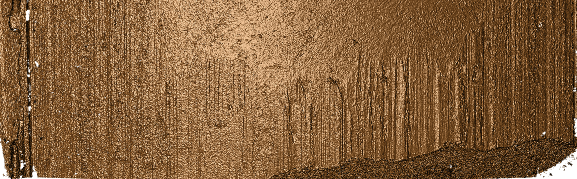
\includegraphics[width=\textwidth]{images/B6-B2-L6.png}

\begin{center}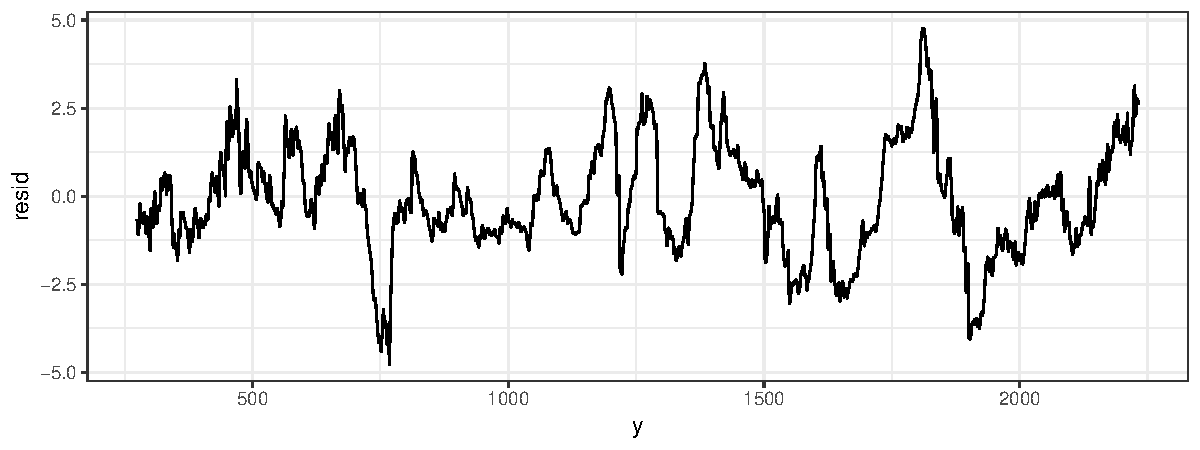
\includegraphics[width=\textwidth]{figures/unnamed-chunk-1-1} \end{center}

\caption{\label{fig:rgl} Image of a bullet land from a confocal light microscope at 20 fold magnification.}

\end{figure}

\subsection{The Chumbley Score Test}\label{the-chumbley-score-test}

\hh{You need to distinguish between $x(t)$ and $x(t_1)$ - $x(t)$ is a spatial process for some $t$. $x(t_1)$ is the realization of the process in $t_1$. - Alternatively you could also follow the notation in Hadler et al on 'digitized toolmarks at a pixel level' - where our 'pixel' is the resolution of the confocal light microscope, i.e. a pixel corresponds to 0.645 microns.}

The Chumbley score algorithm takes input as two vectorized processes
\(x(t_1)\) and \(y(t_2)\) which denote two sets of marks or striae.
These marks or striae are potentially from two different bullets or two
different toolmarks whose source needs to be identified as being same or
different. The marks or striae are indexed by the pixel location where
\(t_1\) is for the first striae referred to as \(x\) and \(t_2\) is for
the second striae which is referred as \(y\). \(t_1\) and \(t_2\) need
not be the same but are usually of similar lenghtsThe similarity is then
judged by the algorithm on the basis of cross-correlation of a fixed and
constant number consecutive pixels say \(k\) taken from the two indexed
marks \(x(t_1)\) and \(y(t_2)\) such that in theory \(k\) remains
smaller that length of the two striae or marks which is the same as
\(t_1\) and \(t_2\). Depending on the what stage of the algorithm we are
in, matching of different pixel lengths and locations is done, which at
the end effectively compares all possible windows that would guarantee
in quantifying the two marks or striae as coming from the same source or
not, which also lets us assess the error rates by checking for a large
number of cases.

The algorithm works in two phases, namely, an optimization step and a
validation step, at the end of which a Mann Whitney U statistic is
calculated. A pre-processing step to the algorithm is to choose a
coarseness value which is used as a parameter to the LOWESS smoothing
function. The coarseness essentially gives the proportion of points
which influence the smooth at each value, which means larger values lead
to more smoothness. The LOWESS smoothing is applied to each of two sets
of vectorized striae or marks \(x(t_1)\) and \(y(t_2)\), before
proceeding to the algorithm.

\citet{hadler} in their paper proposed an improvement to this algorithm
by trying to remove mutual dependence of parameters (due to serial
correlation in surface depth values of a toolmark and because of a
random sampling sub step in the validation phase which makes a group of
pixels to be chosen more than once and hence introduces lack of
independence) in certain steps, especially because the Mann-Whitney U
statistic that is later calculated in the algorithm and used as a
measure to differentiate between matches and non-matches works under the
assumption of independence of parameters.

Since we are only interested in a non-parameteric U statistic, Hadler et
al. proposed a normalization procedure in the Validation step that goes
to some extent to address the issue of mutual dependence. Also the same
shift and different shift substep was modified to use a deterministic
rule for sampling sam-shhift and dofferent shift-samples as opposed to
the originally proposed random samples.

The data that is used by \citet{chumbley} is generated by a surface
profilometer that gives the height in terms of distance along a linear
trace. This is taken perpendicular to the striations present in the
toolmark. Two such trace are then compared using the algorithm.

\subsection{Detailed algorithm}\label{detailed-algorithm}

\subsubsection{Optimization step}\label{optimization-step}

The idea behind this step is to first identify the area of best
agreement in the two toolmark data. Comparison window size is predefined
by the user, which in case of screwdriver toolmarks was chosen by
Chumbley et al and Hadler et al as around 10 percent of the length of
the toolmarks, which was around 500. This window is henceforth referred
to as Window of optimization.

A maximum correlation statistic is used to identify the region of best
agreement, with the maximum usually seen being near 1 for both cases
which is what we intuitively expect for matches, and something which we
do not intuitively expect for non matches
\gk{done}\hh{XXX get rid of the parentheses - put the content into a sentence after your first statement.}

\hh{XXX the process you describe below is the cross-correlation of two series $x(t)$ and $y(t)$.}

First, there are a very large number of cross-correlations calculated
for the two series of striae or marks \(x(t_1)\) and \(y(t_2)\), for eg
if the window of optimization was defined as 200 and toolmark pixel
length is around 1000 then we have 1200-(200-1) = 1001. Can be thought
of ordered arrangements without replacement where n = 1001 and r = 1.

This is the number of windows we have for one toolmark and each window
is compared with all windows of the second toolmark (the number of
windows is again similar), and the window with the maximum correlation
is identified to be the region where the toolmarks are in maximum
agreement with each other

\subsubsection{Validation Step}\label{validation-step}

\paragraph{Same-shift:}\label{same-shift}

In this step a series of windows are chosen at random (originally by
chumbley et al) and deterministically (by hadler et al), but at a common
distance (rigid-shift) from the window identified as the region of best
agreement in the vaildation step. The correlation of these windows would
be as intuitively assumed i.e.~lower than the maximum correlation window
(Optimization step), but the significance is that these same shift
windows will still have large enough correlation values for two
toolmarks or signatures that are in reality a match.

This also validates that if in the optimization step the maximum
correlation window chosen (with correlation value near 1) was by
accident (like in case of signatures that in reality are a non-match),
all these same- shift correlations (A fixed number of these trace
segments are identified) would not be anywhere large enough for all
same-shift windows.

\begin{verbatim}
  Classification Match Non-Match
1          Match    47         3
2      Non-Match     0        50
\end{verbatim}

\begin{figure}

{\centering 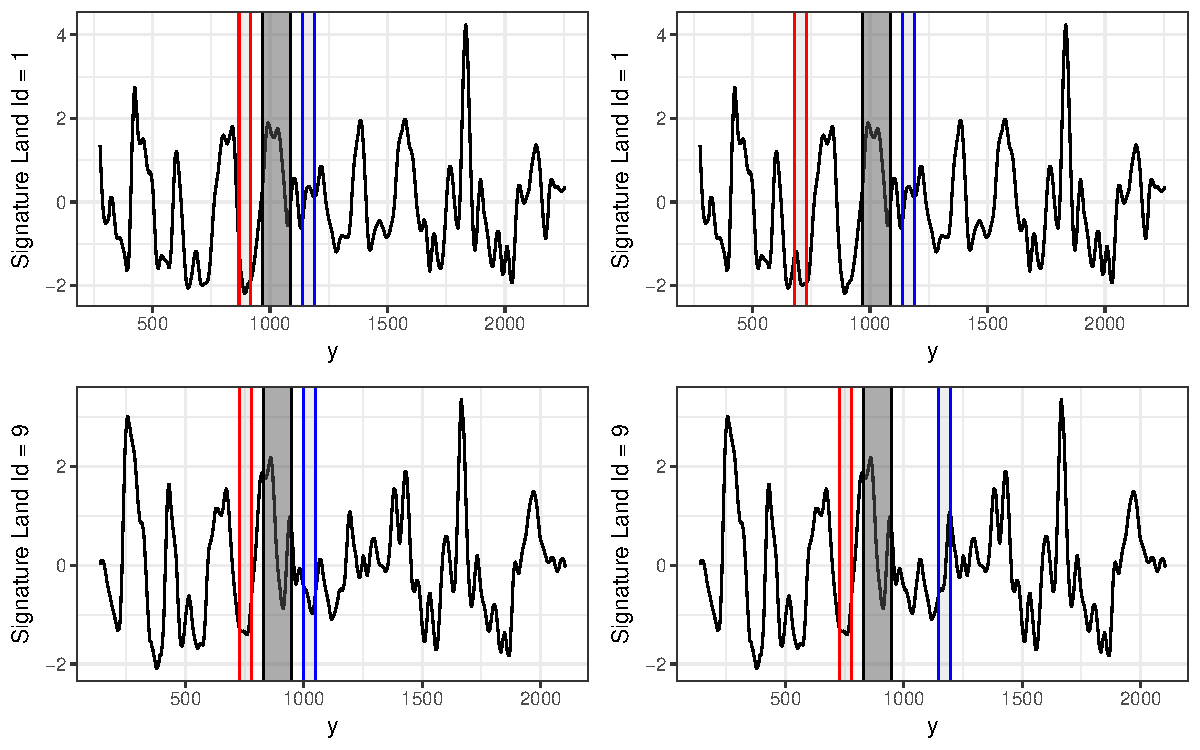
\includegraphics[width=\textwidth]{figures/win-comparison-1} 

}

\caption{ The two plots on the left show how the same shift behaves in case of a matching pair and the two plots on the right show how the different shift behaves in case of a matching pair.}\label{fig:win-comparison}
\end{figure}

\paragraph{Different Shift:}\label{different-shift}

Primary reason for this substep is to give perspective to the
correlation values of the same shift window correlation values.

This time there are no rigid-shifts but different shifts (distance from
Window of Opt with max correlation) chosen randomly by \citet{chumbley}
and deterministically by Hadler et al. such that there is an equal
possibilty of comparing a trace segment from one signature or toolmark
to any one in the second signature or toolamrk.

Neither of above sets of correlation are allowed to include the maximum
correlation window as identified earlier.

Therefore the assumption is that if two toolmarks or signatures match
each other the same-shift correlations would be larger than the
different-shift windows, and if they are not a match the correlations in
the two sets will be very similar.

\subsubsection{U Statistic:}\label{u-statistic}

This is computed from the joint rank of all correlations of both the
same and different shift samples. As given by \citet{hadler}

Null Hypothesis: If the toolmarks were not match i.e not made by the
same tool.

Let ns and nd be the number of same shift and different shift windows
\(N = n_{s} + n_{d}\)

The mann whitney U statistic is given by
\(U =\sum^{ns}_{i=1}R_{s}\left( i\right)\)

with the standardized version which includes provision for rank ties

\(\overline{U}= \dfrac{U-M}{\sqrt{V}}\)

where prior to normalization the U-statistic has the mean as

\(M = n_{s}\left(\dfrac{N+1}{2}\right)\)

and variance

\(V = \dfrac{n_{s}n_{d}}{N\left(N-1\right)}\left[\Sigma^{n_{s}}R_{s}\left(i\right)^{2}+\Sigma^{n_{d}}R_{d}\left(j\right)^{2}\right] -\dfrac{n_{s} n_{d}\left(N+1\right)^{2}}{4\left(N-1\right)}\)

\subsection{Potential limitations of the Chumbley
Score}\label{potential-limitations-of-the-chumbley-score}

\hh{in the application to striation marks on bullet lands: smaller in width and curved - need to adjust parameter settings; something similar is done in \citet{afte-chumbley} for toolmark comparisons of slip-joint pliers. XXX work in }

Bullets are much smaller in length, width, are not flat and curved in
the cross-sectional topography as opposed to tools like screw driver
tips which produced longer and pronounced markings. This means the
makings made by barrels in comparison to toolmarks may have a problem in
distinctiveness. The majority of Bullet profiles and signatures
extracted by procedures mentioned by \citet{aoas} are almost 1/4 th the
size of toolmarks as used by \citet{chumbley} or even smaller.
Striations on Bullets are made on their curved surfaces, whereas the
algorithm developed by \citet{chumbley} and \citet{hadler} has only been
tested for flatter and wider surfaces which have negligible curvature.
Therefore, using methods proposed for toolmarks may need adaptation in
order to give tangible results for bullets. Moreover, in order to to get
flat bullet signatures and remove the curvatures some kind of smoothing
needs to be applied as a pre-step which needs further investigation as
to whether the level of smoothing does effect the working of the
algorithm on Bullets.

Also when in the optimization step, the Window of optimization for
bullets will be shorter as the signatures are smaller. The idea is to
keep the number of windows of optimization sufficiently large, which
means shorter Trace segments (partition of signature or toolmark with
length = size of window of optimization) that lets us compare smaller
segments of one signature to another.

This introduces a problem as, if we go too small in the window of
optimization, the unique features of the trace segments are lost and
seem similar, while too large sizes vastly reduces the weight of small
features that would otherwise uniquely classify a signature and hence
identify the region of agreement.

Thus the Window of Optimization has a direct influence on whether we are
Falsely rejecting the null when it is true (Type I) or Falsely accepting
the null when it is false (Type II) making identification of the optimum
size of window of optimization very important.

\subsection{Testing setup:}\label{testing-setup}

\hh{Using cross-validation setup to identify appropriate parameter settings for (a) signatures and (b) profiles directly}

Following on similar lines to the setup of toolmarks, the first step
here is to first identify what difference does different window sizes of
optimization and the validation step have, when adapting the toolmark
method to bullets.

The marking made on bullets are smaller than toolmarks and is also less
wider. The idea is to find out possible areas of error while adapting
the score based method proposed for toolmarks.

Bullet signatures being compared at this time are from the Hamby 44 and
Hamby 252 data, which have the best set of known-matched and known
non-matches.

Bullet signatures are chosen by 1. Filtering out Land\_id for Profiles
from the Hamby 44 and Hamby 252 data and removing all NA values 2.
run\_id = 3 is chosen, Seems like the signatures generated from this
run\_id give the closest match. Different run\_id's have some different
settings for generating the signatures (The level of smoothing does not
seem to be one of them)

The bullet signatures when generated already included the LOWESS
smoothing. Therefore, the coarseness factor is set to 1 while running
the chumbley\_non\_random() which generates the same\_shift,
different\_shift, U-Stat and P\_value parameters.

\begin{table}[!h]

\caption{\label{tab:unnamed-chunk-2}Window of Optimization 320 and Window of Validation 50}
\centering
\begin{tabular}[t]{lrr}
\toprule
  & FALSE & TRUE\\
\midrule
FALSE & 77564 & 412\\
TRUE & 4022 & 674\\
\bottomrule
\end{tabular}
\end{table}

\begin{table}[!h]

\caption{\label{tab:unnamed-chunk-3}Window of Optimization 120 and Window of Validation 50}
\centering
\begin{tabular}[t]{lrr}
\toprule
  & FALSE & TRUE\\
\midrule
FALSE & 78938 & 371\\
TRUE & 4281 & 845\\
\bottomrule
\end{tabular}
\end{table}

\begin{table}[!h]

\caption{\label{tab:unnamed-chunk-4}Window of Optimization 80 and Window of Validation 50}
\centering
\begin{tabular}[t]{lrr}
\toprule
  & FALSE & TRUE\\
\midrule
FALSE & 78817 & 450\\
TRUE & 4680 & 775\\
\bottomrule
\end{tabular}
\end{table}

\section{Results}\label{results}

\subsection{Signatures}\label{signatures}

Signatures of lands for all Hamby-44 and Hamby-252 scans made available
through the NIST ballistics database \citep{nist} were considered. Both
of these sets of scans are part of the larger Hamby study \citep{hamby}
and each consist of twenty known bullets (two each from ten
consecutively rifled Ruger P85 barrels) and fifteen questioned bullets
(each matching one of the ten barrels). Ground truth for both of these
Hamby sets is known and was used to assess correctness of the tests
results.

We used the adjusted Chumbley method as proposed in \citet{hadler} and
implemented in the R package \texttt{toolmaRk} \citep{toolmark} on all
pairwise land-to-land comparisons of the Hamby scans (a total of 85,491
comparisons) in the following manner:

\begin{table}[!h]

\caption{\label{tab:unnamed-chunk-5}Overview of parameter settings used for optimization and validation windows for bullet land signatures.}
\centering
\resizebox{\linewidth}{!}{\begin{tabular}[t]{lrrrrrrrrrrrrrrrrr}
\toprule
wo & 50 & 50 & 60 & 60 & 80 & 80 & 90 & 90 & 100 & 100 & 110 & 110 & 120 & 120 & 120 & 120 & 120\\
wv & 30 & 50 & 30 & 50 & 30 & 50 & 30 & 50 & 30 & 50 & 30 & 50 & 10 & 20 & 30 & 50 & 60\\
\bottomrule
\end{tabular}}
\end{table}

\begin{table}[!h]
\centering
\resizebox{\linewidth}{!}{\begin{tabular}{lrrrrrrrrrrrrrrrrr}
\toprule
wo & 120 & 130 & 130 & 140 & 140 & 150 & 150 & 160 & 160 & 200 & 200 & 200 & 240 & 240 & 280 & 280 & 320\\
wv & 60 & 30 & 50 & 30 & 50 & 30 & 50 & 30 & 50 & 20 & 30 & 50 & 30 & 50 & 30 & 50 & 50\\
\bottomrule
\end{tabular}}
\end{table}

\subsubsection{Signatures}\label{signatures-1}

Figure \ref{fig:type2} gives an overview of type II error rates observed
when varying the window size in the optimization step.

\begin{figure}

{\centering 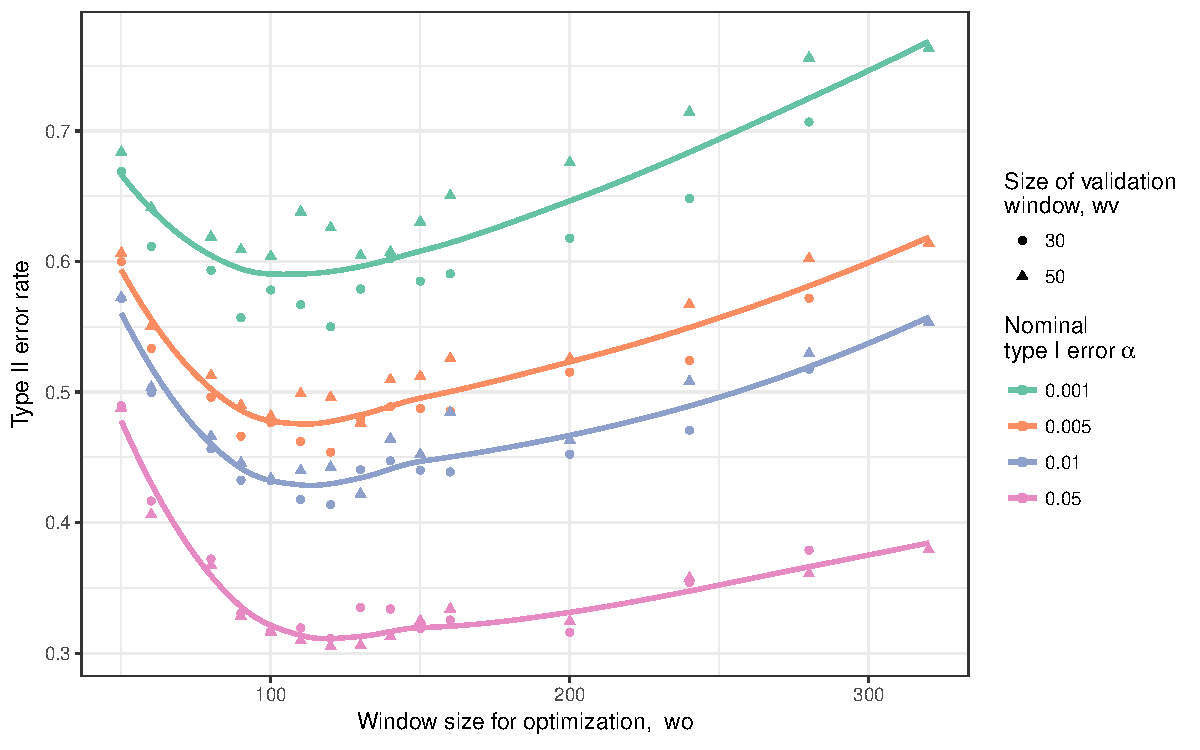
\includegraphics[width=\textwidth]{figures/type2-1} 

}

\caption{Type II error rates observed across a range of window sizes for optimization $wo$. For a window size of $wo = 120$ we see a drop in type II error rate across all type I rates considered. Smaller validation sizes $wv$ are typically associated with a smaller type II error.}\label{fig:type2}
\end{figure}

Figure \ref{fig:type1} compares nominal (fixed) type I error and
actually observed type I errors for the parameter settings in table XXX.
With an increasing size of the window used in the optimization step the
observed type I error rate decreases (slighty). This might be related to
the increasing number of tests that fail for larger window sizes, in
particular for non-matching striae (see fig \ref{fig:missings}).

\begin{figure}

{\centering \includegraphics[width=\textwidth]{figures/type1-1} 

}

\caption{Comparison of observed and nominal type I error rates  across a range of window sizes for optimization $wo$. The horizontal line in each facet indicates the nominal type I error rate.  As the optimization window increase the observed type I error rate gets smaller. A smaller validation window tends to be associated with a higher type I error rate.}\label{fig:type1}
\end{figure}

\begin{figure}

{\centering 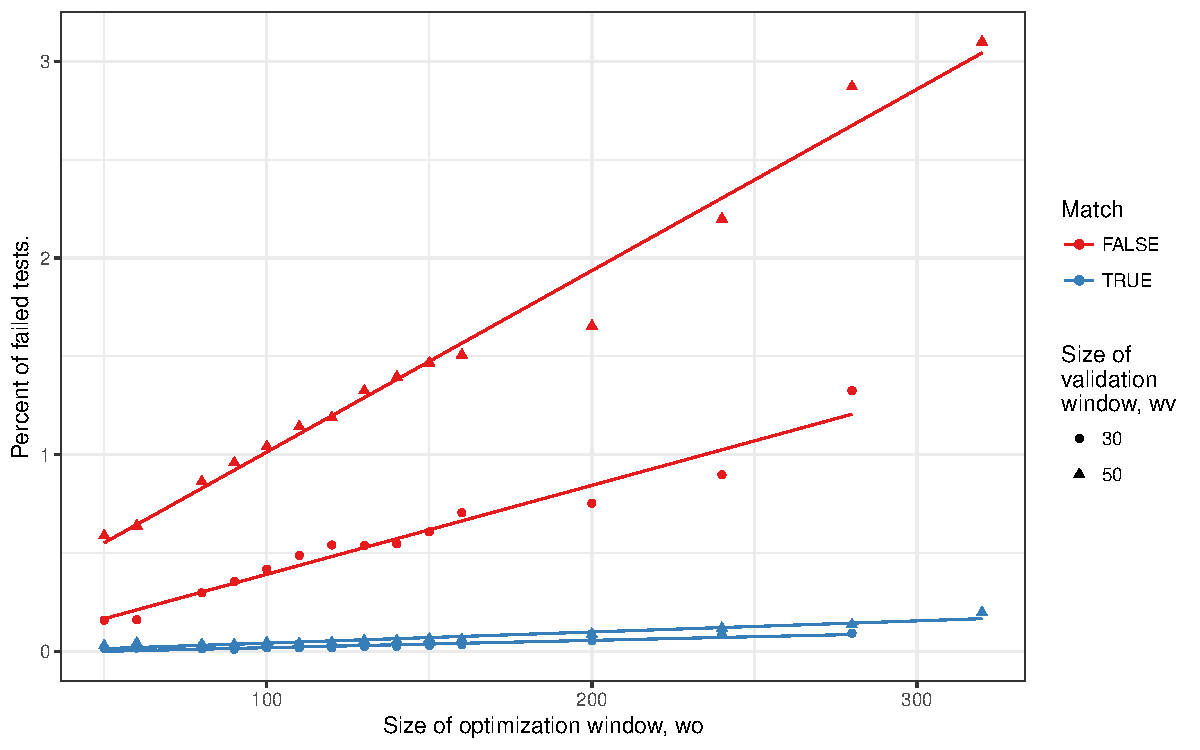
\includegraphics[width=\textwidth]{figures/missings-1} 

}

\caption{Number of failed tests by the window optimization size, wo, and ground truth. Test results from different sources have a much higher chance to fail, raising the question, whether failed tests should be treated as rejections of the null hypothesis of same source.}\label{fig:missings}
\end{figure}

Figure \ref{fig:missings} gives an overview of the number of failed
tests, i.e.~tests in which a particular parameter setting did not return
a valid result. This happens, when the shift to align two signatures is
so large, that the remaining overlap is too small to accommodate windows
for validation. The problem is therefore exacerbated by a larger
validation window. Figure \ref{fig:missings} also shows that the number
of failed tests is approximately linear in the size of the optimization
window.

\begin{table}

\caption{\label{tab:lms}Estimates of the increase in percent of failed tests corresponding to a 100 point increase in the optimization window.}
\centering
\begin{tabular}[t]{lrrr}
\toprule
match & wv & estimate & std.error\\
\midrule
FALSE & 30 & 0.452 & 0.027\\
FALSE & 50 & 0.922 & 0.035\\
TRUE & 30 & 0.037 & 0.004\\
TRUE & 50 & 0.056 & 0.005\\
\bottomrule
\end{tabular}
\end{table}

\begin{center}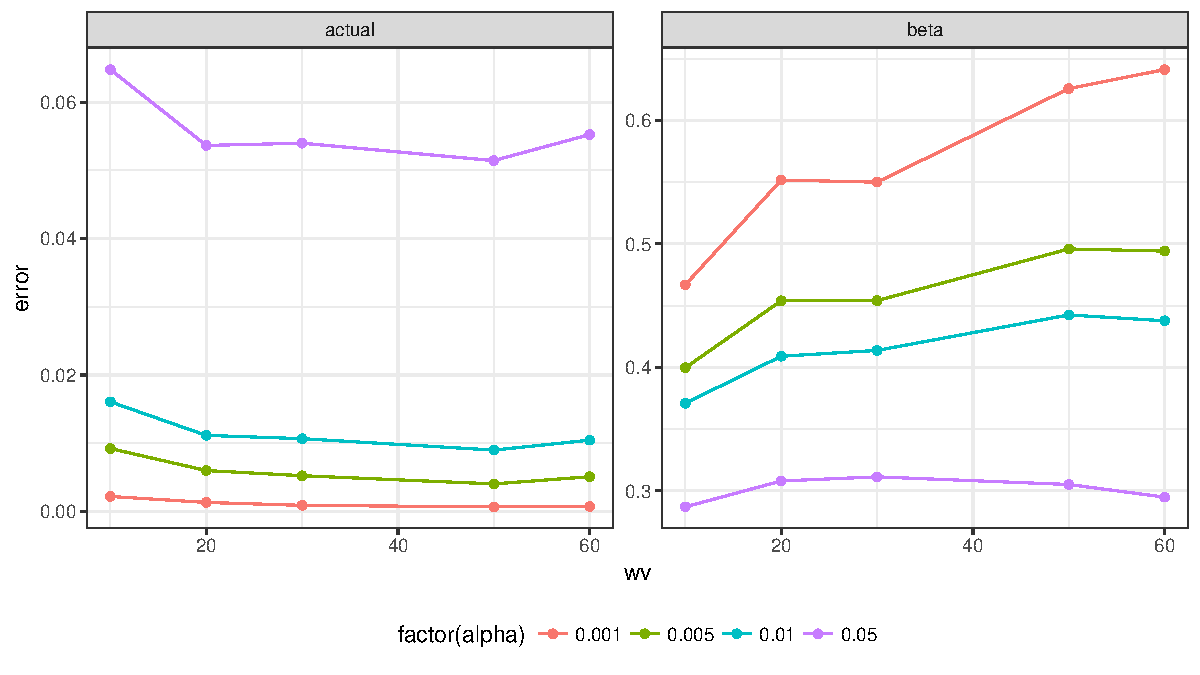
\includegraphics[width=\textwidth]{figures/wo120-1} \end{center}

\subsubsection{Profiles}\label{profiles}

The profiles are cross-sectional values of the the bullet striation mark
which are chosen at an optimum height (x as used by \citet{aoas}). This
x or height is not a randomly chosen level. The rationale behind the
choice has been explained by \citet{aoas}. A region is first chosen
where the cross-correlation seems to change very less and in this region
an optimum height is chosen. The profiles generally resemble a curve
which is more or less similar to a quadratic curve (a quadratic fit to
the raw data values of the profile is not an exact fit but it does show
a similar trend). Profiles are the set of raw values representing the
striation marks, and signatures are generated from these by removal of
the inherent curvature and applying some smoothing (the signatures
generated by \citet{aoas} use a loess function for smoothing).

Coming back to the database of Hamby-44 and Hamby-252 datasets, the
run\_id = 3 was used when applying the chumbley algorithm on the
signatures. The run\_id not only defines the level of smoothing but also
signifies the chosen height at which the profiles were selected
initially. Another important aspect is the range of horizontal values
(which is referred to as the y values in \citet{aoas}) in the
signatures. Thes have already been pre-processed in the database to not
include any grooves.

Therefore for the sake of comparison the run\_id = 3 is still chosen so
as to ensure that the horizontal values remain the same as that of the
signatures. This also gives us profiles with the grooves removed.

\hh{XXX ideas should go to the previous section on setting up the study; in this section we focus on results only XXX}
The idea therefore is to first use these raw values of the profile
directly in the chumbley algorithm, and see how the algorithm performs
for different coarseness values (smoothing parameter as referred in the
function LOWESS used in the chumbley algorithm)

\begin{figure}

{\centering 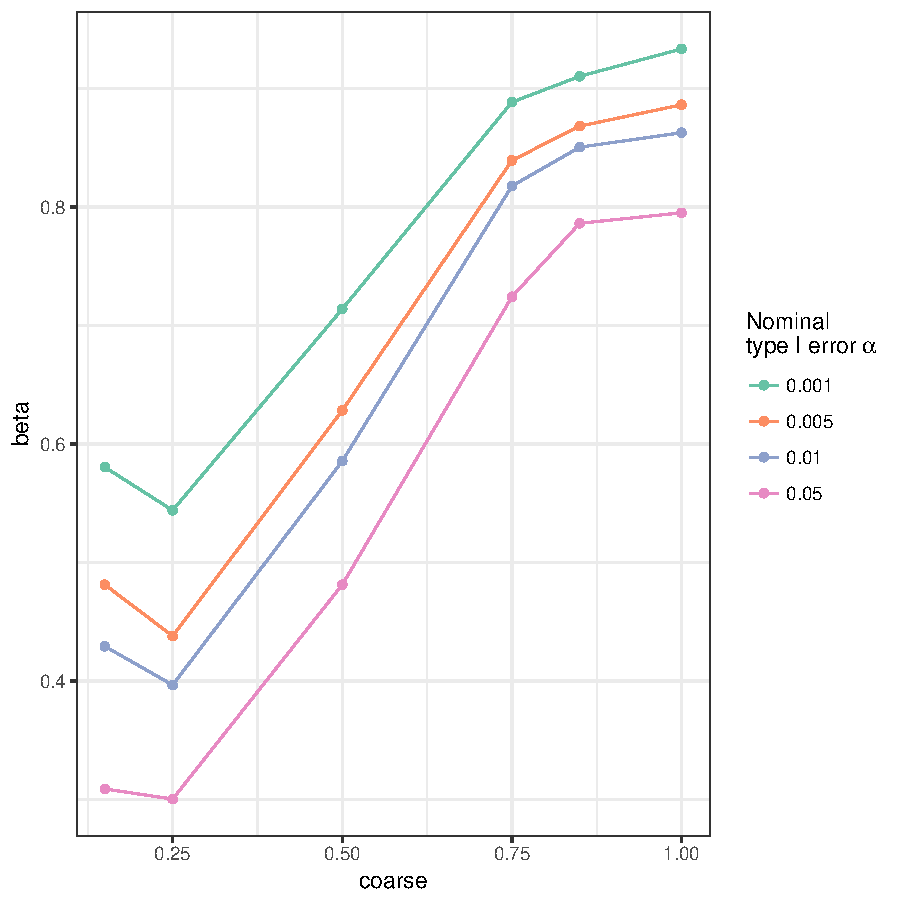
\includegraphics[width=\textwidth]{figures/unnamed-chunk-6-1} 

}

\caption{Type II errors for different levels of coarseness. XXX We need more values around .25}\label{fig:unnamed-chunk-6}
\end{figure}

\subsubsection{comparison of total error with signatures and
profiles}\label{comparison-of-total-error-with-signatures-and-profiles}

\begin{center}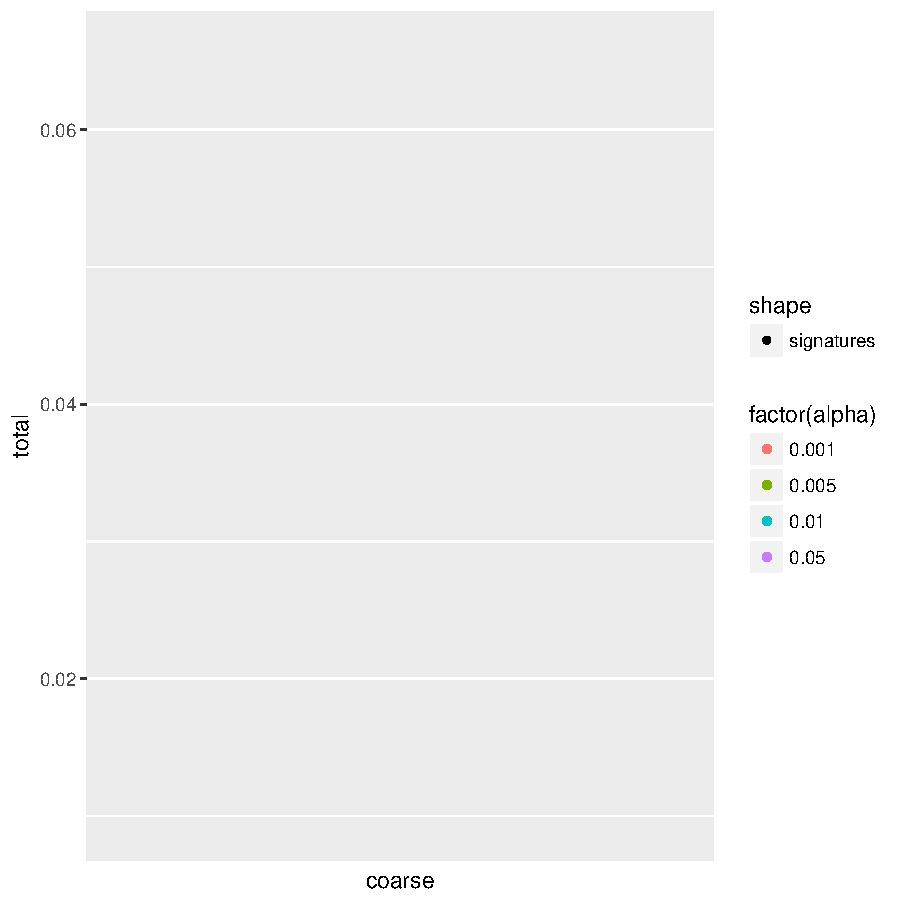
\includegraphics[width=\textwidth]{figures/unnamed-chunk-7-1} \end{center}

\subsection{Discussion}\label{discussion}

\subsection{Results of Chumbley score}\label{results-of-chumbley-score}

\begin{itemize}
\tightlist
\item
  Nominal alpha value shows dependency on the size of the window of
  optimization
\item
  Test Fail depends on whether known-match or known non-matches has
  predictive value
\item
  Type II error least bad for window of validation 30 and window of
  optimization 120
\end{itemize}

\section{Algorithm Modification}\label{algorithm-modification}

The proposed algorithm modification is at the same shift step which
comes after the shift distance is identified by finding two windows in
the two markings that have the highest correlation.

The modification allows for a ``wiggle'' room in the second marking of
the two sets of markings being compared. This means that each set of
same shift windows that are being compared, the second marking will
window that is under consideration is allowd to move a little towards
the left and a little towards the right.

This gives us a new set of 4 windows, 2 to the left and 2 to the right
of the original comparison window. Then the correlations for each one of
these 5 windows with the window under consideration of the 1st marking
is retrieved (from the validation step correlation matrix) or computed.

Then the window that has the maximum correlation (from the set of 5
windows in the 2nd marking) with the window of the 1st marking is
chosen.

This new maximum correlation is then used to compute the U-statistics
using the same method as before.

\subsection{Expected advantage of
modification}\label{expected-advantage-of-modification}

We are expecting that this modification would improve the type I and II
errors for the good. Less number of false negatives and false positives.
The reason for this expectation is many a times the bullet markings are
not made at the same distances for two or more bullets because of the
way it comes out of the barrel.

Therefore rigid same shifts might not necessarily compare the right set
of windows. In the same shift step for one set of windows, allowing the
window in the 2nd marking to wiggle left and right and finding the best
match to the window in the 1st marking, lets us adjust for situations
where markings are compressed or elongated.

\subsection{Dependence on the delta of new windows from the original
same shift
window}\label{dependence-on-the-delta-of-new-windows-from-the-original-same-shift-window}

From initial tests the amount of movement to get new windows left and
right of the original same shift window seems to directly influence the
the pvalue and U statistic that we look at.

\subsubsection{other questions}\label{other-questions}

How much movement is reasonable and should be used? Is there a way to
understand if the 2nd marking in comparison to the 1st marking is
compressed or elongated or neither? Should the amount of movement
selected depend on this compression or elongation? or using a static
delta movement value justifieable.

\bibliographystyle{agsm}
\bibliography{bibliography}

\end{document}
